\documentclass[11pt,a4paper]{article}
\usepackage[T1]{fontenc}
\usepackage[utf8]{inputenc}
\usepackage[czech]{babel}
\usepackage{amsmath}
\usepackage{amssymb}
\usepackage{booktabs}
\usepackage{geometry}
\geometry{a4paper, margin=2.5cm}
\usepackage{float}
\usepackage{graphicx}
\usepackage{subcaption}
\graphicspath{{figures/}}
\usepackage{listings}
\usepackage{xcolor}

\lstset{
    basicstyle=\ttfamily\small,
    backgroundcolor=\color{gray!10},
    frame=single,
    breaklines=true,
    captionpos=b,
    keywordstyle=\color{blue},
    inputencoding=utf8,
    extendedchars=true,
    literate={á}{{\'a}}1 {é}{{\'e}}1 {í}{{\'i}}1 {ó}{{\'o}}1 {ú}{{\'u}}1 {ý}{{\'y}}1 {č}{{\v{c}}}1 {ď}{{\v{d}}}1 {ě}{{\v{e}}}1 {ň}{{\v{n}}}1 {ř}{{\v{r}}}1 {š}{{\v{s}}}1 {ť}{{\v{t}}}1 {ž}{{\v{z}}}1 {Á}{{\'A}}1 {É}{{\'E}}1 {Í}{{\'I}}1 {Ó}{{\'O}}1 {Ú}{{\'U}}1 {Ý}{{\'Y}}1 {Č}{{\v{C}}}1 {Ď}{{\v{D}}}1 {Ě}{{\v{E}}}1 {Ň}{{\v{N}}}1 {Ř}{{\v{R}}}1 {Š}{{\v{S}}}1 {Ť}{{\v{T}}}1 {Ž}{{\v{Z}}}1
}

\usepackage{enumitem}
\setlist{noitemsep, topsep=2pt}
\usepackage[hidelinks]{hyperref}

\title{Analýza vlastností kodéru \hyperref[sec:standards]{HEVC} a~moderních alternativ\\
\large B(E)2M37KASA - Komprese obrazu a~signálů}
\author{Tomáš Hurta \and Tomáš Kratochvíle}
\date{\today}

\begin{document}

\maketitle

\begin{abstract}
Tento semestrální projekt se zabývá analýzou a~srovnáním vlastností moderních standardů pro kompresi videa (\hyperref[sec:standards]{HEVC}, \hyperref[sec:standards]{AVC}, \hyperref[sec:standards]{VP9}, \hyperref[sec:standards]{AV1}) pomocí nástroje FFmpeg. Na standardizovaných testovacích sekvencích v~rozlišení 1080p50 je hodnocena efektivita komprese pomocí metrik \hyperref[sec:metrics]{PSNR}, \hyperref[sec:metrics]{SSIM} a~\hyperref[sec:metrics]{VMAF} v~závislosti na datovém toku a~výpočetní náročnosti. Výsledky ukazují, že moderní kodéry jako libx265 a~libsvtav1 dosahují výrazné úspory datového toku oproti staršímu standardu \hyperref[sec:standards]{AVC}, zatímco hardwarová akcelerace na architektuře Apple Silicon nabízí extrémní propustnost (přes 160 \hyperref[sec:derived_metrics]{FPS}) za cenu nárůstu datového toku o~více než 300\ \% pro dosažení shodné percepční kvality.
\end{abstract}

\tableofcontents
\newpage

\section{Úvod}
S~neustálým růstem objemu multimediálních dat na internetu roste i~tlak na efektivitu metod komprese obrazu a~videa. Tento projekt se zaměřuje na praktické srovnání vybraných moderních videokodeků. Důraz je kladen na standard High Efficiency Video Coding (\hyperref[sec:standards]{HEVC}), známý též jako H.265, a~jeho pozici vůči staršímu standardu Advanced Video Coding (\hyperref[sec:standards]{AVC}, H.264) a~moderním alternativám \hyperref[sec:standards]{VP9} a~\hyperref[sec:standards]{AV1}. Cílem práce je demonstrovat vlastnosti těchto kodeků pomocí softwaru FFmpeg, detailně popsat jejich kompresní efektivitu a~analyzovat vliv použitého hardwaru na výsledný poměr kvality a~datového toku. Veškeré měřicí skripty, vygenerovaná data a~zdrojové kódy tohoto dokumentu jsou veřejně dostupné v~repozitáři na platformě GitHub \href{https://github.com/kratot17/KASA_SEM}{(kratot17/KASA\_SEM)}. Složky s~objemnými daty, konkrétně nekomprimovaná referenční videa (\texttt{raw\_videos}) a~vygenerované výstupy z~kodérů (\texttt{encoded\_videos}), jsou z~kapacitních důvodů uloženy v~dedikované složce na \href{https://drive.google.com/drive/folders/1dQosNQVMNARsGfBLjNj08zZU0Cm_nrx5?usp=sharing}{Google Drive}.

\section{Teoretický základ}
\subsection*{Paradigma standardizace videa: Dekodér vs. Kodér}
Zásadním konceptem v~oblasti komprese videa je skutečnost, že mezinárodní standardy (jako H.264 či \hyperref[sec:standards]{HEVC}) specifikují výhradně syntaxi datového toku (\hyperref[sec:glossary]{bitstream}) a~proces dekódování. Každý standardizovaný dekodér musí ze stejného bitstreamu vyprodukovat identický obraz. Proces \textit{kódování} (encoding) však standardizován není. Výrobci hardwaru a~tvůrci softwaru mají volnou ruku v~tom, jaké heuristiky a~optimalizační algoritmy použijí, pokud je výsledkem validní \hyperref[sec:glossary]{bitstream}. Z~tohoto důvodu se vlastnosti různých kodérů implementujících stejný standard diametrálně liší v~kvalitě, rychlosti i~hardwarové náročnosti.

\subsection*{Standardy a~softwarové kodéry}
\label{sec:standards}
Pro účely práce byly zvoleny následující video standardy a~k~nim příslušné softwarové implementace kodérů dostupné v~knihovně FFmpeg:

\begin{itemize}
    \item \textbf{H.264 (\hyperref[sec:standards]{AVC}) a~\texttt{libx264}:} Standard z~roku 2003, aktuálně nejrozšířenější formát na světě s~téměř 100\% hardwarovou kompatibilitou na přehrávacích zařízeních. Poskytuje excelentní rovnováhu mezi rychlostí enkódování a~kvalitou.
    \item \textbf{H.265 (\hyperref[sec:standards]{HEVC}) a~\texttt{libx265}:} Nástupce \hyperref[sec:standards]{AVC}. Přinesl koncept \textit{Coding Tree Units} (CTU) o~velikosti až 64x64 pixelů (oproti fixním 16x16 macroblokům v~H.264) a~35 směrů intra-predikce (oproti 9 v~H.264) \cite{lec_hevc}. Zavádí také technologii \textit{Sample Adaptive Offset} (SAO) pro potlačení artefaktů na hranách a~redukci tzv. ringing efektu \cite{lec_hevc}. Díky těmto vylepšením dosahuje až 50\% úspory datového toku vůči H.264 při zachování stejné kvality.
    \item \textbf{\hyperref[sec:standards]{VP9} a~\texttt{libvpx-vp9}:} Otevřená a~bezplatná alternativa k~\hyperref[sec:standards]{HEVC}, masivně využívána platformou YouTube pro streamování 4K videa. Formát VP8 (zmíněný v~zadání) byl z~testování vyloučen, neboť je v~současnosti považován za obsolentní a~byl plně nahrazen technologicky vyspělejším standardem \hyperref[sec:standards]{VP9}.
    \item \textbf{\hyperref[sec:standards]{AV1} a~\texttt{libsvtav1}:} Formát vyvinutý aliancí AOMedia. Nabízí mimořádně efektivní kompresi, jejíž jedinou nevýhodou je extrémní výpočetní náročnost omezující její nasazení v~reálném čase.
\end{itemize}

\subsection*{Konfigurace a~použití nástroje FFmpeg}
Pro zajištění reprodukovatelnosti experimentu uvádíme klíčové parametry použité pro kódování. Je nutné zdůraznit, že parametr \hyperref[sec:glossary]{CRF} (Constant Rate Factor) není mezi různými kodéry přímo srovnatelný (např. \hyperref[sec:glossary]{CRF} 22 u~x264 neprodukuje stejnou kvalitu jako \hyperref[sec:glossary]{CRF} 22 u~\hyperref[sec:standards]{AV1}). Hlavním nástrojem pro srovnání efektivity jsou proto R-D křivky.

Použité konfigurace:
\begin{itemize}
    \item \textbf{x264/x265:} \texttt{-preset medium} (výchozí kompromis mezi rychlostí a~efektivitou).
    \item \textbf{\hyperref[sec:standards]{VP9}:} \texttt{-deadline good -cpu-used 2} (standardní režim pro \hyperref[sec:glossary]{VOD}).
    \item \textbf{\hyperref[sec:standards]{AV1}:} \texttt{-preset 8} (vyvážené nastavení pro moderní CPU).
    \item \textbf{HW \hyperref[sec:standards]{HEVC}:} \texttt{-q:v~[60, 66, 72, 78]} (ekvivalenty kvality pro Apple Silicon).
\end{itemize}

\begin{lstlisting}[language=bash, caption={Příklad příkazu pro kódování do \hyperref[sec:standards]{HEVC} (CPU vs. HW).}]
# Softwarové kódování (libx265)
ffmpeg -y -i~input.y4m -c:v~libx265 -preset medium -crf 28 output_cpu.mp4

# Hardwarově akcelerované kódování (Apple Silicon)
ffmpeg -y -i~input.y4m -c:v~hevc_videotoolbox -q:v~72 output_hw.mp4
\end{lstlisting}

Výpočet objektivních metrik byl realizován pomocí komplexního filtru (\texttt{-lavfi}) integrovaného přímo ve FFmpeg, který v~jednom průchodu generuje logy pro PSNR, SSIM a~VMAF.

\begin{lstlisting}[language=bash, caption={Příklad příkazu pro výpočet metrik \hyperref[sec:metrics]{PSNR}, \hyperref[sec:metrics]{SSIM} a~\hyperref[sec:metrics]{VMAF}.}]
ffmpeg -i~encoded.mp4 -i~reference.y4m -lavfi "[0:v][1:v]psnr=stats_file=psnr.log;[0:v][1:v]ssim=stats_file=ssim.log;[0:v][1:v]libvmaf=n_threads=8:log_path=vmaf.csv:log_fmt=csv" -f null -
\end{lstlisting}

\subsection*{Metriky objektivní kvality videa}
\label{sec:metrics}
Pro vyhodnocení dopadu ztrátové komprese využíváme tři základní metriky srovnávající referenční a~komprimovaný obraz:

\begin{itemize}
    \item \textbf{\hyperref[sec:metrics]{PSNR} (Peak Signal-to-Noise Ratio):} Měří podíl mezi maximální hodnotou signálu a~chybou (\hyperref[sec:glossary]{MSE}). Ačkoliv je standardně používána, její korelace s~lidským vnímáním je omezená, neboť nereflektuje sémantický obsah obrazu \cite{lec_iqa, wang2004image}.
    \item \textbf{\hyperref[sec:metrics]{SSIM} (Structural Similarity Index):} Hodnotí zachování strukturální informace (hran a~textur), luminanci a~kontrast. Skóre se pohybuje v~intervalu od 0 do 1.
    \item \textbf{\hyperref[sec:metrics]{VMAF} (Video Multi-Method Assessment Fusion):} Metrika vyvinutá společností Netflix \cite{netflixVMAF}. Pomocí algoritmů strojového učení se snaží simulovat lidského diváka a~aproximovat subjektivní hodnocení MOS (Mean Opinion Score). Pro výpočet byl použit standardní model pro Full HD (1080p) sledování ze vzdálenosti televizního přijímače. Skóre nabývá hodnot od 0 do 100.
\end{itemize}

\subsection*{Odvozené technické a~efektivnostní metriky}
\label{sec:derived_metrics}
Analýza výkonnosti kodérů se neopírá pouze o~obrazovou kvalitu, ale i~o~analytické metriky odvozené z~velikosti souborů a~času zpracování. 

\textbf{Kompresní poměr (Compression Ratio - \hyperref[sec:derived_metrics]{CR})} definuje poměr mezi původní nekomprimovanou velikostí dat ($S_{orig}$) a~velikostí zkomprimovaného souboru ($S_{comp}$):
\begin{equation*}
    \hyperref[sec:derived_metrics]{CR} = \frac{S_{orig}}{S_{comp}}
\end{equation*}

\textbf{Bits Per Pixel (\hyperref[sec:derived_metrics]{BPP})} je metrika nezávislá na rozlišení určující průměrný počet bitů alokovaných na jeden pixel obrazu, kde $R$ je datový tok, $W$ šířka, $H$ výška a~$\hyperref[sec:derived_metrics]{FPS}$ snímková frekvence:
\begin{equation*}
    \hyperref[sec:derived_metrics]{BPP} = \frac{R}{W \times H \times \hyperref[sec:derived_metrics]{FPS}}
\end{equation*}

\textbf{Rychlost kódování v~\hyperref[sec:derived_metrics]{FPS}} poskytuje přesnější údaj o~výpočetní propustnosti kodéru než prostý časový údaj, zejména při porovnávání různě dlouhých videí:
\begin{equation*}
    FPS_{enc} = \frac{N_{frames}}{t_{enc}}
\end{equation*}

\section{Metodika práce}

\subsection*{Příprava pracovního prostředí a~filozofie testování}
Proces testování byl proveden lokálně na jednom stroji: Apple MacBook Pro osazený čipem M1 Pro. Během celého procesu kódování a~výpočtu metrik byl počítač trvale připojen k~napájecímu zdroji, aby se předešlo jakémukoli podtaktování či omezení výkonu.

Smyslem práce není stanovit absolutní časy enkódování (které by se lišily s~každou další generací procesorů), ale zkoumat poměrové metriky – porovnávat výstupy a~náročnost algoritmů \textit{relativně vůči sobě} za identických podmínek na jediném zařízení.

\subsection*{Specifikace testovacích videí}
Jako referenční bod byla stažena nekomprimovaná videa z~databáze Xiph.org \cite{xiphDerf}. Zvolené sekvence reprezentují náročné kompresní scénáře.
\begin{itemize}
    \item \textbf{Formát a~prostor:} \hyperref[sec:glossary]{Y4M} (YUV4MPEG2), bez komprese. Barevný prostor \hyperref[sec:glossary]{YUV 4:2:0}, 8-bit.
    \item \textbf{Rozlišení a~frekvence:} 1920x1080 (Full HD) při 50 snímcích za sekundu (fps).
    \item \textbf{Objem dat a~kompresní poměr:} Všechna referenční videa mají délku 10 sekund (500 snímků). Vzhledem k~absenci komprese je jejich velikost na disku přesně identická, a~to \textbf{1~555~203~036 bajtů} (cca 1555,20 MB).
    \item \textbf{Prostorová složitost:} Pro objektivní zhodnocení náročnosti jednotlivých scén byla změřena průměrná Shannonova entropie jasové složky (Y) všech snímků referenčních videí (viz Tabulka \ref{tab:entropy}). Tato hodnota indikuje míru prostorové redundance (\textit{Spatial Redundancy}) v~sekvenci, kterou se kodéry snaží eliminovat \cite{lec_tech}.
\end{itemize}

\begin{figure}[H]
    \centering
    \begin{subfigure}[b]{0.32\textwidth}
        \centering
        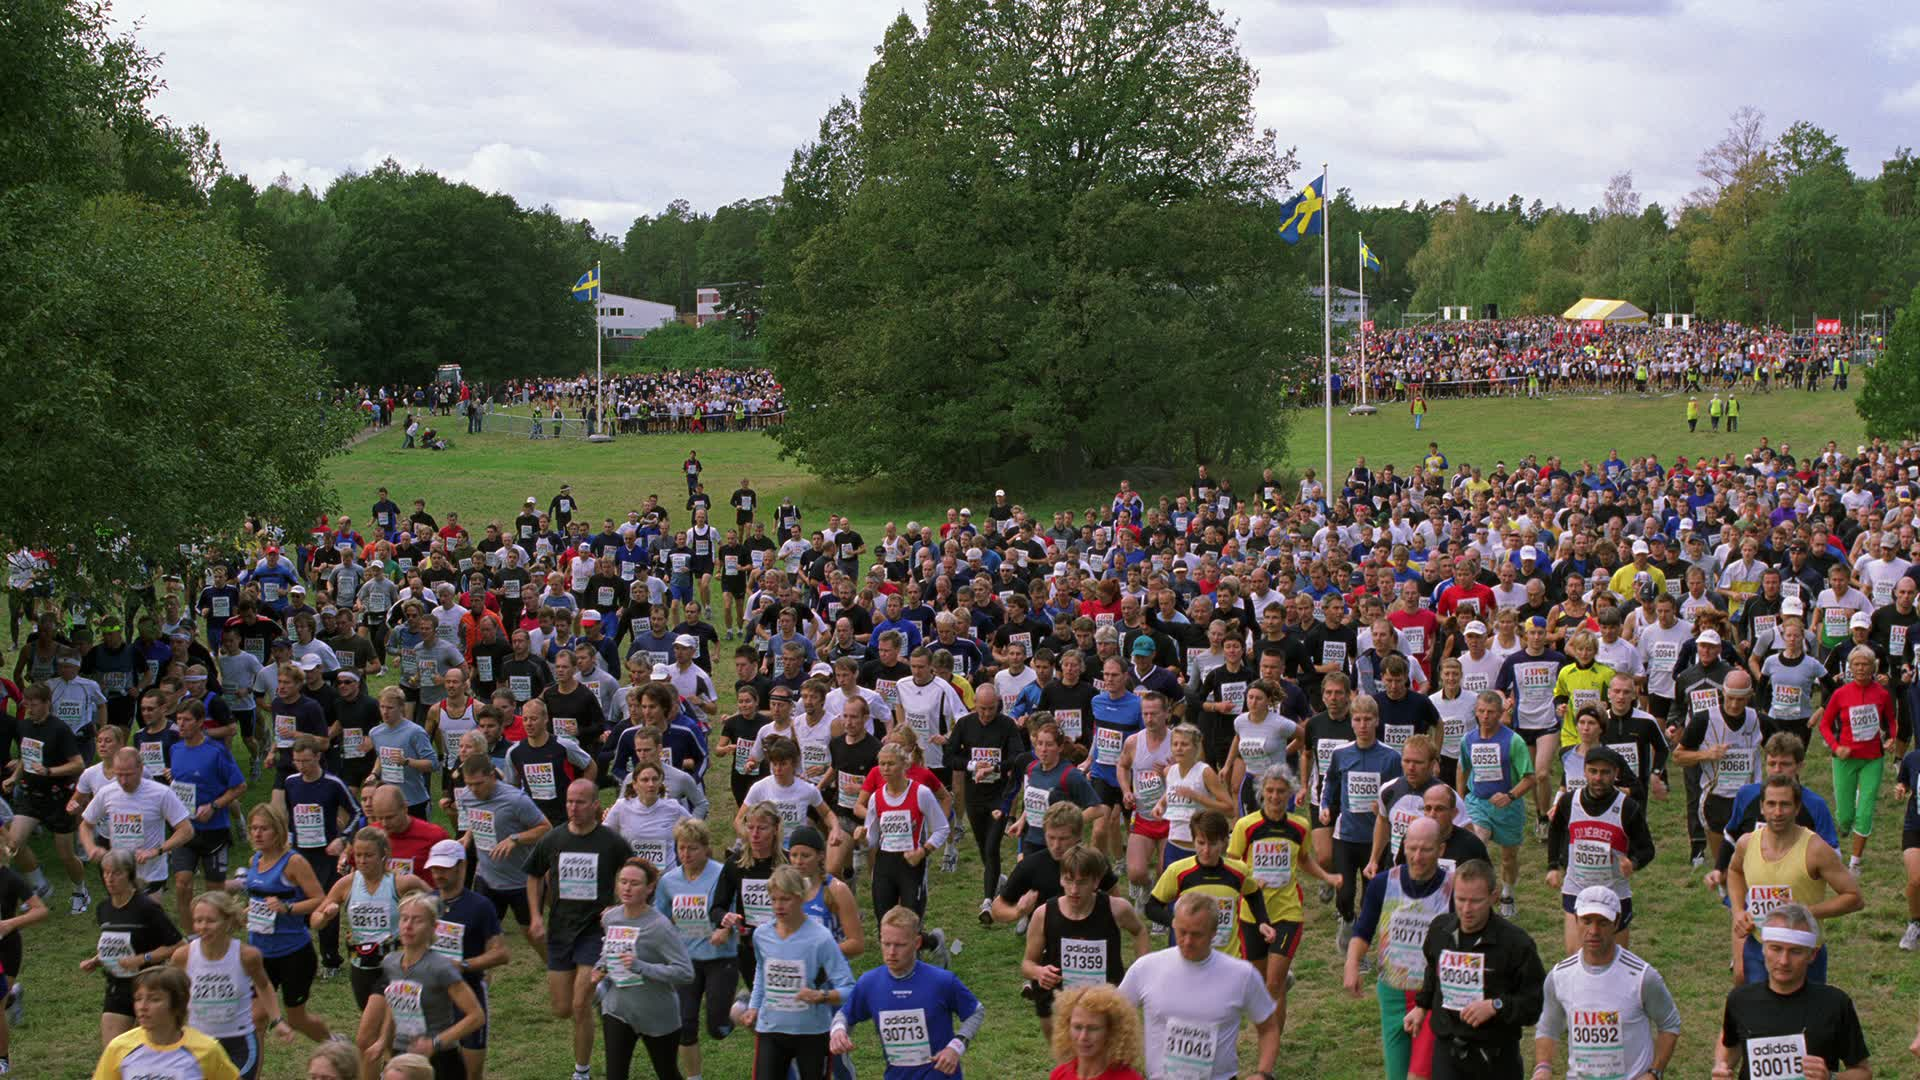
\includegraphics[width=\textwidth]{frame_crowd_run.jpg}
        \caption{crowd\_run}
    \end{subfigure}
    \hfill
    \begin{subfigure}[b]{0.32\textwidth}
        \centering
        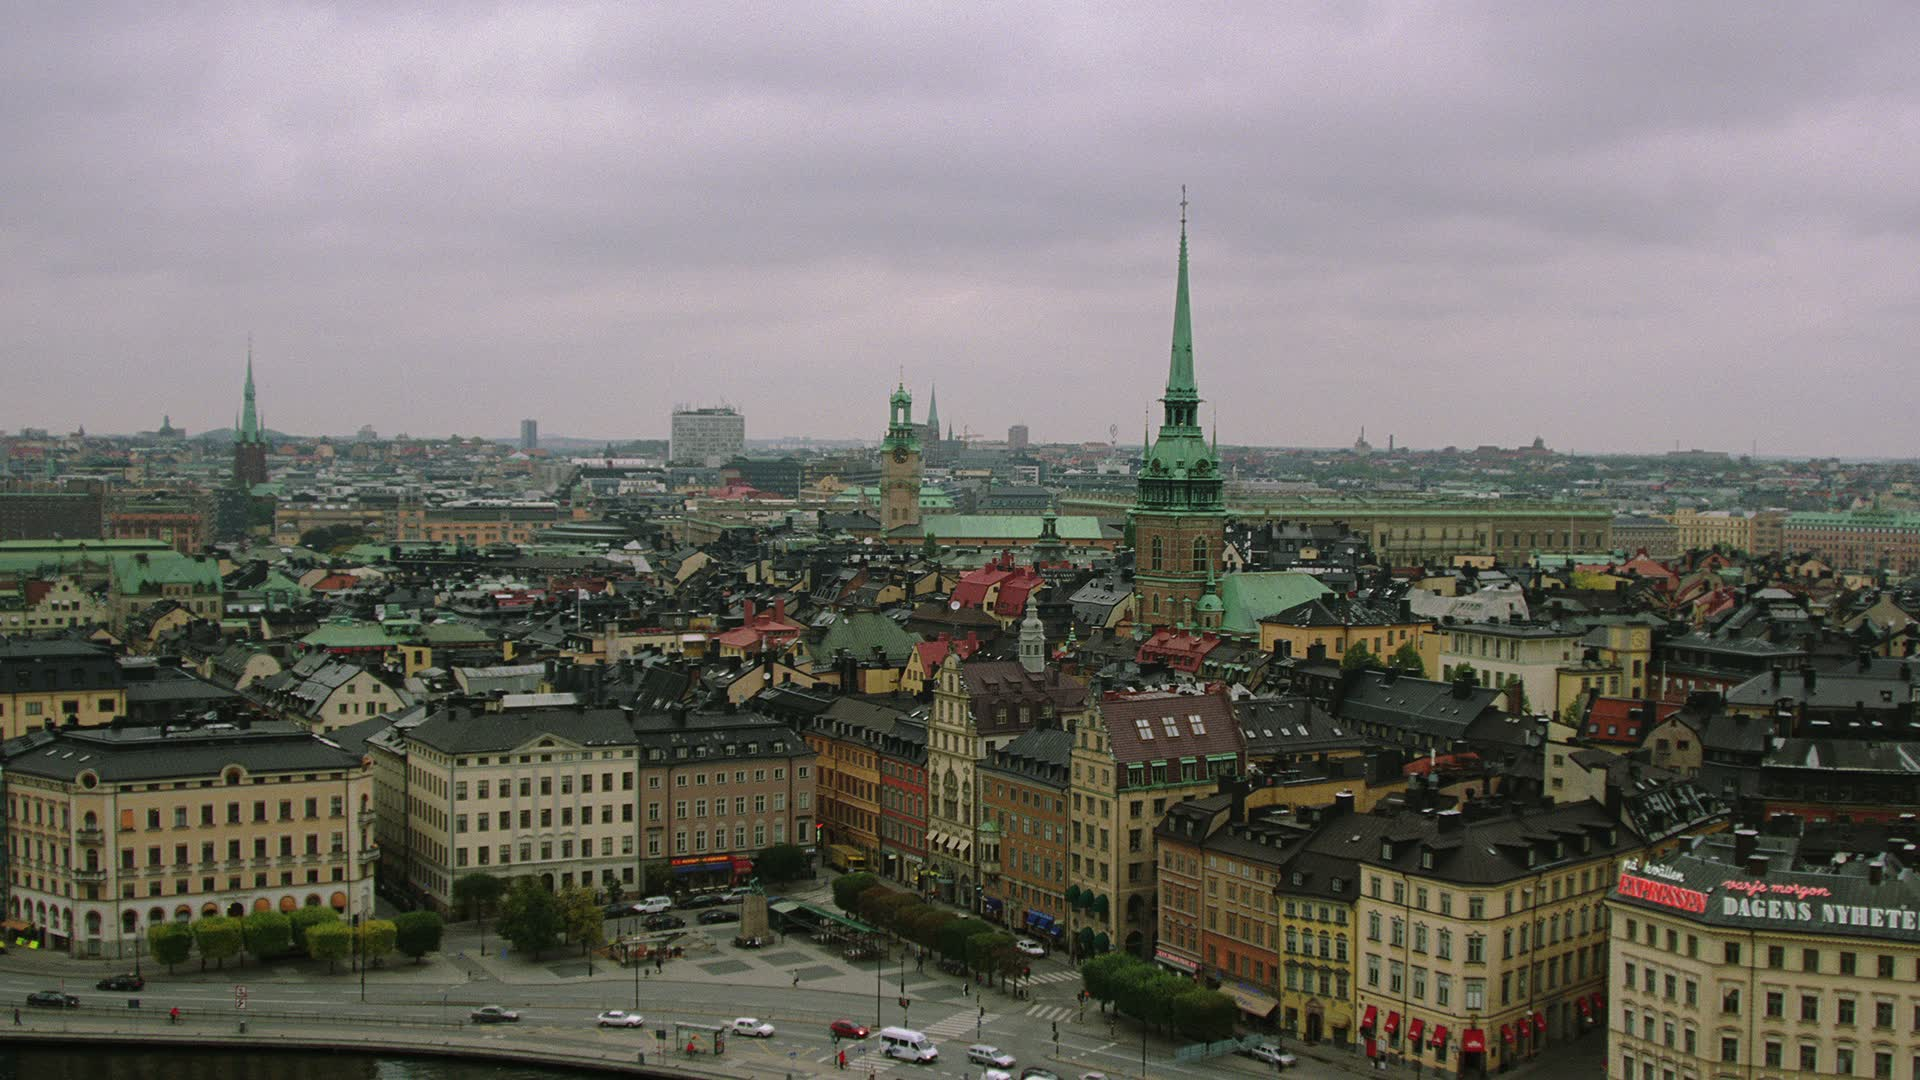
\includegraphics[width=\textwidth]{frame_old_town.jpg}
        \caption{old\_town\_cross}
    \end{subfigure}
    \hfill
    \begin{subfigure}[b]{0.32\textwidth}
        \centering
        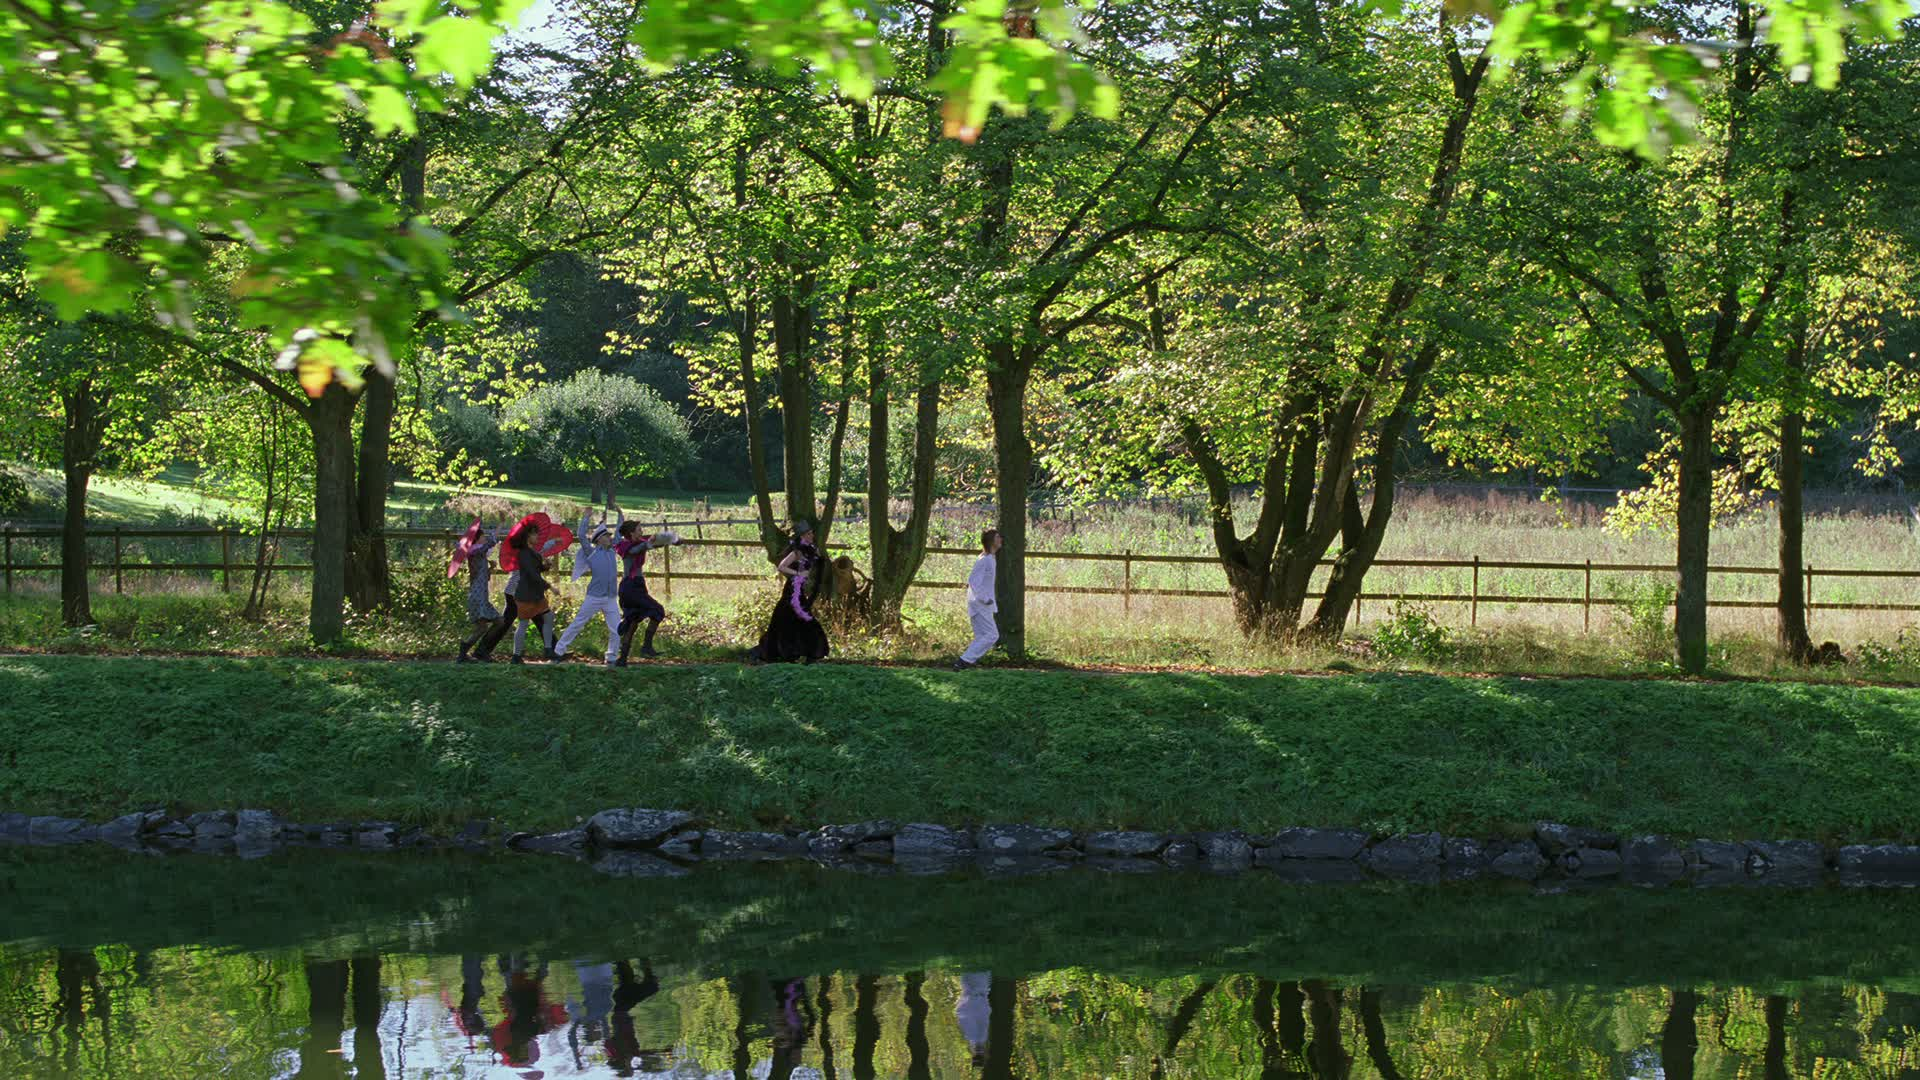
\includegraphics[width=\textwidth]{frame_park_joy.jpg}
        \caption{park\_joy}
    \end{subfigure}
    \caption{Ukázkové snímky (250. snímek) z~použitých testovacích sekvencí v~rozlišení 1080p.}
    \label{fig:frames_showcase}
\end{figure}

\begin{table}[H]
\centering
\caption{Naměřená prostorová entropie referenčních video sekvencí.}
\label{tab:entropy}
\begin{tabular}{|l|c|c|c|}
\hline
\textbf{Testovací sekvence} & \textbf{Prům. entropie [bit/px]} & \textbf{Min} & \textbf{Max} \\
\hline
crowd\_run\_1080p50.y4m & 7,4464 & 7,1432 & 7,6512 \\
old\_town\_cross\_1080p50.y4m & 7,1095 & 6,9841 & 7,2354 \\
park\_joy\_1080p50.y4m & 6,9707 & 6,8512 & 7,0921 \\
\hline
\end{tabular}
\end{table}

\subsection*{Dávkové zpracování (FFmpeg)}
Pomocí skriptu byl aplikován software FFmpeg \cite{ffmpeg}. Úroveň kvality byla řízena pomocí parametru \hyperref[sec:glossary]{CRF} (pro softwarové kodéry) a~parametru \texttt{q:v} (pro HW). Testovány byly kompromisní stupně kvality s~ohledem na odlišné implementace škálování. 

\section{Výsledky a~diskuze}

\subsection*{Výkonnostní srovnání a~vliv HW akcelerace}
V~této sekci uvádíme detailní srovnání výkonnosti pouze pro sekvenci \textit{crowd\_run}. Tato sekvence byla vybrána jako reprezentativní vzorek, neboť vykazuje nejvyšší prostorovou entropii a~je pro kodéry nejnáročnější. Jak je patrné z~doplňujících tabulek v~Příloze \ref{sec:appendix}, relativní rozdíly v~propustnosti (\hyperref[sec:derived_metrics]{FPS}) a~čase mezi jednotlivými kodéry zůstávají u~ostatních videí velmi podobné a~potvrzují stejné trendy – naprostou dominanci hardwarového řešení v~rychlosti a~vyšší analytickou efektivitu softwarových kodérů.

V~Tabulce \ref{tab:times} jsou uvedeny výsledky měření pro scénář s~vysokou vizuální kvalitou (odpovídající nastavení \hyperref[sec:glossary]{CRF} 22). Zde je nejvíce patrný rozdíl mezi softwarovou hloubkou analýzy a~hrubou silou hardwarového enginu.

Zatímco hardwarový kodér \texttt{hevc\_videotoolbox} dosahuje extrémní propustnosti (přes 160 \hyperref[sec:derived_metrics]{FPS}), jeho neschopnost provádět komplexní optimalizace vede k~tomu, že pro stejnou úroveň vizuální kvality vyžaduje výrazně vyšší datový tok. Tento propad efektivity u~\hyperref[sec:glossary]{ASIC} (Application-Specific Integrated Circuit) enginu je způsoben zejména omezeným rozsahem hledání pohybu (Motion Search) a~absencí nebo silným omezením B-snímků (Bi-directional frames) v~rámci GOP (Group of Pictures). To potvrzuje naměřený nárůst datového toku o~více než 300\ \% ve srovnání s~\texttt{libx265} při shodné úrovni \hyperref[sec:metrics]{VMAF}.

\begin{table}[H]
\centering
\caption{Srovnání výkonnosti kodérů pro vysokou kvalitu obrazu (vstup: 500 snímků, 1080p50, sekvence crowd\_run). Kompletní tabulky pro ostatní sekvence jsou v~Příloze \ref{sec:appendix}.}
\label{tab:times}
\begin{tabular}{|l|c|r|r|r|c|}
\hline
\textbf{Kodér} & \textbf{\hyperref[sec:derived_metrics]{FPS}} & \textbf{Čas [s]} & \textbf{Původní [MB]} & \textbf{Komprim. [MB]} & \textbf{Úspora} \\
\hline
hevc\_videotoolbox (HW) & 166,67 & 3 & 1555,20 & 182,31 & 88,28\ \% \\
libx264 (CPU) & 62,50 & 8 & 1555,20 & 35,13 & 97,74\ \% \\
libx265 (CPU) & 25,00 & 20 & 1555,20 & 42,28 & 97,28\ \% \\
libsvtav1 (CPU) & 41,67 & 12 & 1555,20 & 110,49 & 92,90\ \% \\
libvpx-vp9 (CPU) & 4,81 & 104 & 1555,20 & 126,70 & 91,85\ \% \\
\hline
\end{tabular}
\end{table}

\subsection*{Analýza objektivity R-D křivek}
Účelem vyhodnocení Rate-Distortion (R-D) křivek je znázornit vztah mezi datovým tokem (zde reprezentovaným velikostí souboru) a~naměřenou kvalitou obrazu. Efektivnější kodér demonstruje strmější křivku, která se posouvá více nahoru a~doleva.

Na Obrázku \ref{fig:rd_vmaf_crowd} je vidět aplikace metriky \hyperref[sec:metrics]{VMAF} na pohybově složitou sekvenci. Potvrzuje se efektivita nejnovějšího standardu \hyperref[sec:standards]{AV1} (\texttt{libsvtav1}). Hardwarový kodér je v~této grafické reprezentaci výrazně posunut vpravo; vyžaduje přibližně čtyřnásobný objem dat k~udržení stejného \hyperref[sec:metrics]{VMAF} skóre jako \texttt{libx265}. 

\begin{figure}[H]
    \centering
    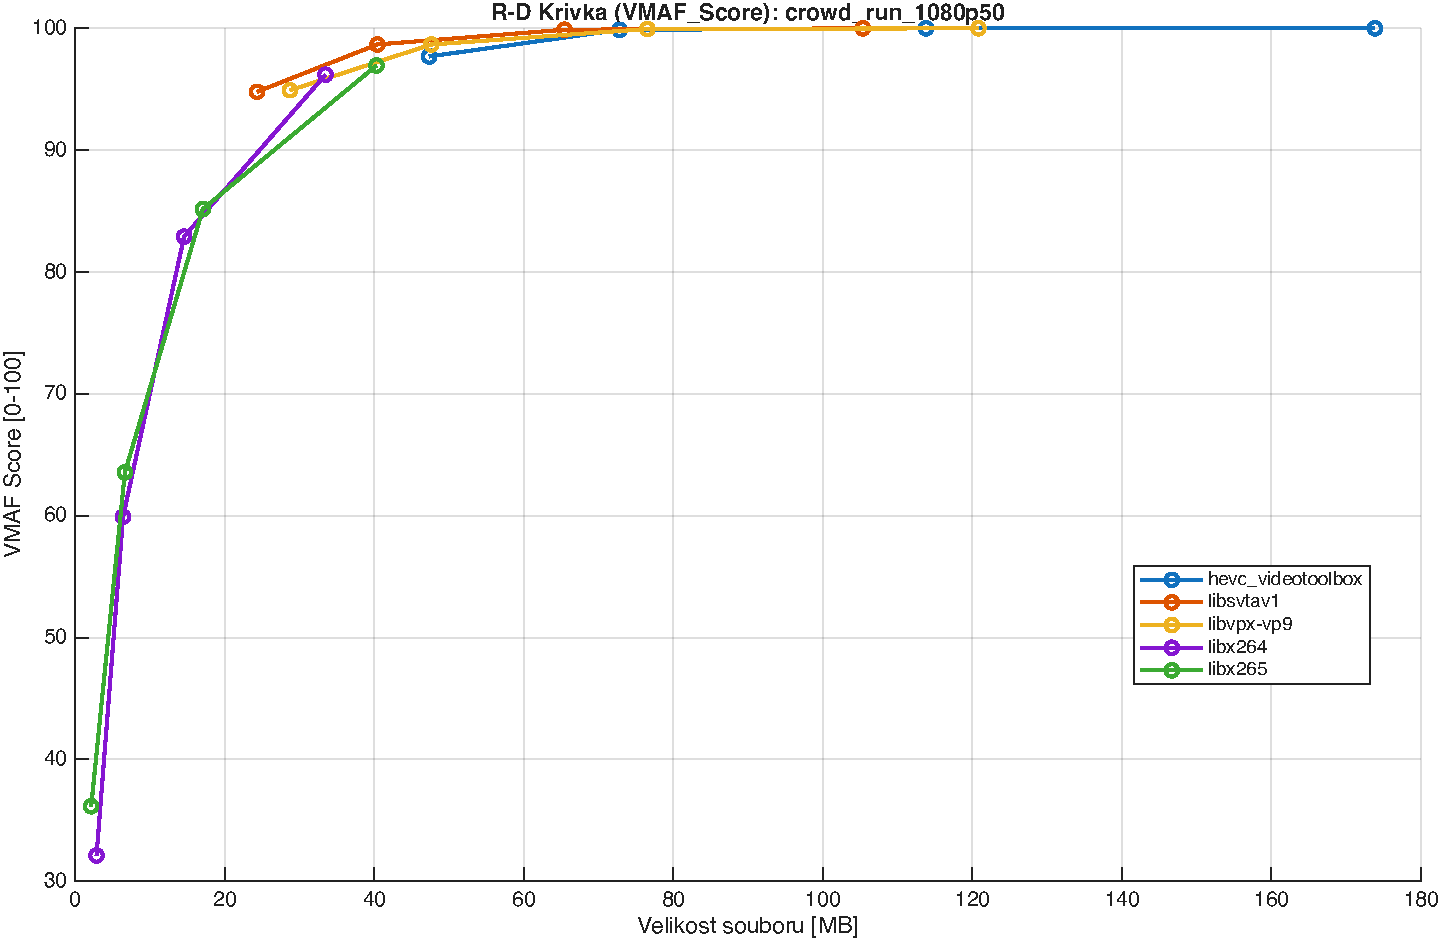
\includegraphics[width=0.8\textwidth]{rd_vmaf_crowd_run_1080p50.pdf}
    \caption{R-D Křivka (\hyperref[sec:metrics]{VMAF}) pro sekvenci crowd\_run\_1080p50.}
    \label{fig:rd_vmaf_crowd}
\end{figure}

\subsection*{Vliv prostorové složitosti a~časová stabilita}
Z~naměřených výsledků vyplývá přímá úměra mezi prostorovou složitostí (entropií) a~kompresní náročností. Sekvence \textit{crowd\_run}, vykazující nejvyšší entropii (7,45 bit/px), vyžaduje pro dosažení \hyperref[sec:metrics]{VMAF} skóre 95 u~kodéru \texttt{libx265} o~42 \% vyšší datový tok než sekvence \textit{park\_joy} s~nižší entropií (6,97 bit/px). Tímto se experimentálně potvrzuje teoretický předpoklad o~vlivu prostorové redundance (\textit{Spatial Redundancy}) na efektivitu komprese.

Kromě průměrných hodnot jsme zkoumali i~stabilitu kvality v~čase. Jak ukazuje Obrázek \ref{fig:temporal_vmaf}, při nastavení nominálně „střední“ kvality (CRF 34 / Q 66) se naplno projevuje nekompatibilita škály CRF mezi různými standardy. Zatímco u~\hyperref[sec:standards]{VP9}, \hyperref[sec:standards]{AV1} a~hardwarového \hyperref[sec:standards]{HEVC} představuje tato hodnota stále téměř bezztrátovou kompresi s~obrovským datovým tokem (plochá křivka držící se u~VMAF 100), kodéry \texttt{libx264} a~\texttt{libx265} při CRF 34 již velmi agresivně šetří data. U~nich se kvalita propadá k~hodnotám 60--65 a~na křivce je ostře patrný typický „pilovitý“ průběh (sawtooth pattern), způsobený pravidelným vkládáním kvalitních referenčních (I) snímků, mezi kterými se kvalita predikovaných snímků postupně snižuje.

\begin{figure}[H]
    \centering
    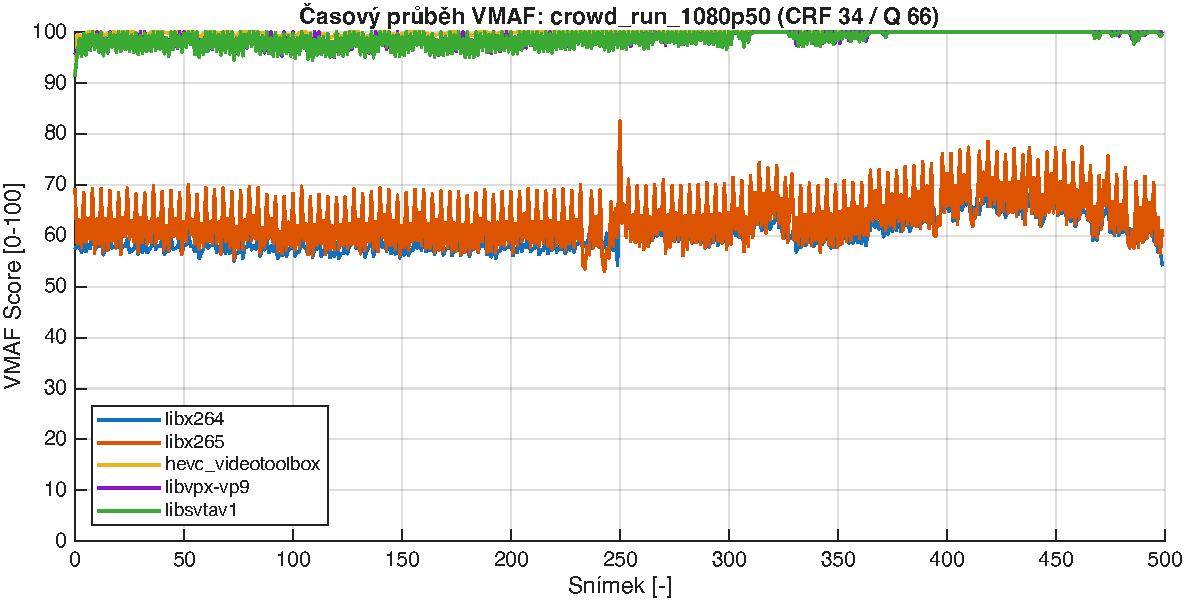
\includegraphics[width=0.85\textwidth]{per_frame_vmaf_crowd_run_1080p50.pdf}
    \caption{Časový průběh \hyperref[sec:metrics]{VMAF} pro sekvenci crowd\_run (střední kvalita).}
    \label{fig:temporal_vmaf}
\end{figure}

Křivky pro další testovací sekvence vykazují analogický trend, kompletní sady naměřených křivek (\hyperref[sec:metrics]{PSNR}, \hyperref[sec:metrics]{SSIM}, \hyperref[sec:metrics]{VMAF} pro všechny testovací sekvence) jsou z~důvodu rozsahu přesunuty do Přílohy na konci dokumentu.

\section{Závěr}
Experimentálně se potvrdilo, že kompresní efektivita úzce souvisí se zvoleným standardem a~optimalizací kodéru. Formáty nové generace (\hyperref[sec:standards]{HEVC} a~\hyperref[sec:standards]{AV1}) bezpečně překonávají dlouholetý standard H.264 z~pohledu úspory dat při zachování percepční kvality. Z~hlediska metriky BD-Rate vykazuje \hyperref[sec:standards]{AV1} (\texttt{libsvtav1}) průměrně o~15--20\ \% nižší datový tok pro dosažení stejného \hyperref[sec:metrics]{VMAF} skóre jako \hyperref[sec:standards]{HEVC} (\texttt{libx265}) v~oblastech s~vysokou kvalitou. Hardwarová akcelerace sice naprosto dominuje v~rychlosti kódování, nicméně aktuální architektura dedikovaných enginů (Apple M1 Pro) postrádá analytickou hloubku softwarových kodérů, což vede k~výrazně nižšímu kompresnímu poměru a~objemnějším souborům (nárůst bitrate o~více než 300\ \% vůči softwarovému \hyperref[sec:standards]{HEVC}).

\newpage
\section*{Slovník pojmů}
\label{sec:glossary}
\addcontentsline{toc}{section}{Slovník pojmů}
\begin{description}
    \item[ASIC (Application-Specific Integrated Circuit):] Integrovaný obvod navržený přesně pro jeden specifický účel, nikoli pro obecné výpočty (jako centrální procesor).
    \item[Bitstream:] Souvislý sled bitů vytvořený procesem komprese (kodérem), který obsahuje data potřebná pro zpětnou rekonstrukci obrazu a~zvuku.
    \item[CRF (Constant Rate Factor):] Režim kódování, který dynamicky alokuje více bitů do složitých scén a~ubírá u~scén statických za účelem udržení konstantní vizuální kvality.
    \item[Y4M (YUV4MPEG2):] Jednoduchý souborový formát, který uchovává zcela nekomprimovaná obrazová data a~doplňuje je o~elementární hlavičku. 
    \item[YUV 4:2:0:] Barevný model separující jas (Y) od barvy (U, V). Podvzorkování 4:2:0 znamená redukci barevné informace na čtvrtinu vůči informaci jasové.
    \item[VOD (Video on Demand):] Služba umožňující uživatelům sledovat video obsah (filmy, seriály) podle vlastního výběru v~libovolném čase, nikoliv podle fixního vysílacího schématu (např. Netflix, YouTube).
    \item[MSE (Mean Squared Error):] Střední kvadratická chyba. Matematická metrika kvantifikující průměrný rozdíl mezi hodnotami pixelů původního a~komprimovaného obrazu. Čím nižší je MSE, tím jsou si obrazy podobnější.
\end{description}

\newpage
\begin{thebibliography}{9}
\sloppy
\addcontentsline{toc}{section}{Reference}

\bibitem{sullivan2012overview}
G. J. Sullivan, J. Ohm, W. -J. Han a~T. Wiegand, \textit{Overview of the High Efficiency Video Coding (\hyperref[sec:standards]{HEVC}) Standard}, in IEEE Transactions on Circuits and Systems for Video Technology, vol. 22, no. 12, pp. 1649-1668, Dec. 2012.

\bibitem{wang2004image}
Z. Wang, A. C. Bovik, H. R. Sheikh a~E. P. Simoncelli, \textit{Image quality assessment: from error visibility to structural similarity}, in IEEE Transactions on Image Processing, vol. 13, no. 4, pp. 600-612, April 2004.

\bibitem{netflixVMAF}
L. Krasula, \textit{Hodnocení kvality obrazu a~jeho využití pro kompresi videa (NETFLIX)}, hostující přednáška (č. 12) v~předmětu B(E)2M37KASA Komprese obrazu a~signálů. [Online]. ČVUT v~Praze, FEL, 2020. Dostupné z: \url{https://moodle.fel.cvut.cz/course/view.php?id=9933}

\bibitem{xiphDerf}
Xiph.org Foundation, \textit{Derf's~Test Media Collection}, Standardizovaná databáze nekomprimovaného videa. [Online]. Dostupné z: \url{https://media.xiph.org/video/derf/}

\bibitem{ffmpeg}
FFmpeg team, \textit{FFmpeg - A~complete, cross-platform solution}. [Online]. Dostupné z: \url{https://ffmpeg.org/}

\bibitem{lec_hevc}
K. Fliegel, \textit{Standardy kódování videa, MPEG1, MPEG2, H.264/\hyperref[sec:standards]{AVC}, H.265/\hyperref[sec:standards]{HEVC}}, přednáška č. 11 v~předmětu B(E)2M37KASA Komprese obrazu a~signálů. [Online]. ČVUT v~Praze, FEL, 2026. Dostupné z: \url{https://moodle.fel.cvut.cz/course/view.php?id=9933}

\bibitem{lec_iqa}
K. Fliegel, \textit{Ztrátové kódování obrazu, lidský vizuální systém, metody hodnocení kvality obrazu}, přednáška č. 8 v~předmětu B(E)2M37KASA Komprese obrazu a~signálů. [Online]. ČVUT v~Praze, FEL, 2026. Dostupné z: \url{https://moodle.fel.cvut.cz/course/view.php?id=9933}

\bibitem{lec_tech}
K. Fliegel, \textit{Základní techniky kódování videa}, přednáška č. 10 v~předmětu B(E)2M37KASA Komprese obrazu a~signálů. [Online]. ČVUT v~Praze, FEL, 2026. Dostupné z: \url{https://moodle.fel.cvut.cz/course/view.php?id=9933}

\end{thebibliography}

\clearpage
\appendix
\section{Příloha: Naměřené grafy a~doplňující data}
\label{sec:appendix}

Tato příloha obsahuje kompletní sadu naměřených grafů pro všechny testované sekvence a~metriky, které nebyly z~důvodu přehlednosti uvedeny v~hlavní části práce.

\subsection*{Srovnání výkonnosti ostatních sekvencí}
V~této sekci jsou uvedeny tabulky výkonnosti pro zbývající testovací sekvence, které doplňují analýzu v~kapitole 4. Hodnoty potvrzují shodné trendy v~propustnosti a~kompresní efektivitě.

\begin{table}[H]
\centering
\caption{Srovnání výkonnosti kodérů (vstup: 500 snímků, 1080p50, sekvence old\_town\_cross).}
\begin{tabular}{|l|c|r|r|r|c|}
\hline
\textbf{Kodér} & \textbf{\hyperref[sec:derived_metrics]{FPS}} & \textbf{Čas [s]} & \textbf{Původní [MB]} & \textbf{Komprim. [MB]} & \textbf{Úspora} \\
\hline
hevc\_videotoolbox (HW) & 166,67 & 3 & 1555,20 & 145,33 & 90,66\ \% \\
libx264 (CPU) & 83,33 & 6 & 1555,20 & 11,11 & 99,29\ \% \\
libx265 (CPU) & 45,45 & 11 & 1555,20 & 11,75 & 99,24\ \% \\
libsvtav1 (CPU) & 50,00 & 10 & 1555,20 & 43,51 & 97,20\ \% \\
libvpx-vp9 (CPU) & 4,10 & 122 & 1555,20 & 92,71 & 94,04\ \% \\
\hline
\end{tabular}
\end{table}

\begin{table}[H]
\centering
\caption{Srovnání výkonnosti kodérů (vstup: 500 snímků, 1080p50, sekvence park\_joy).}
\begin{tabular}{|l|c|r|r|r|c|}
\hline
\textbf{Kodér} & \textbf{\hyperref[sec:derived_metrics]{FPS}} & \textbf{Čas [s]} & \textbf{Původní [MB]} & \textbf{Komprim. [MB]} & \textbf{Úspora} \\
\hline
hevc\_videotoolbox (HW) & 166,67 & 3 & 1555,20 & 226,34 & 85,45\ \% \\
libx264 (CPU) & 71,43 & 7 & 1555,20 & 43,96 & 97,17\ \% \\
libx265 (CPU) & 22,73 & 22 & 1555,20 & 55,49 & 96,43\ \% \\
libsvtav1 (CPU) & 45,45 & 11 & 1555,20 & 134,56 & 91,35\ \% \\
libvpx-vp9 (CPU) & 4,72 & 106 & 1555,20 & 161,92 & 89,59\ \% \\
\hline
\end{tabular}
\end{table}

\newpage
\subsection*{Časová stabilita kvality (\hyperref[sec:metrics]{VMAF} v~čase)}
Zbývající grafy ukazují stabilitu vizuální kvality snímek po snímku při nastavení CRF 34 (CPU) a~Q 66 (HW). Tyto grafy umožňují identifikovat propady kvality v~náročných pasážích videí.

\begin{figure}[H]
    \centering
    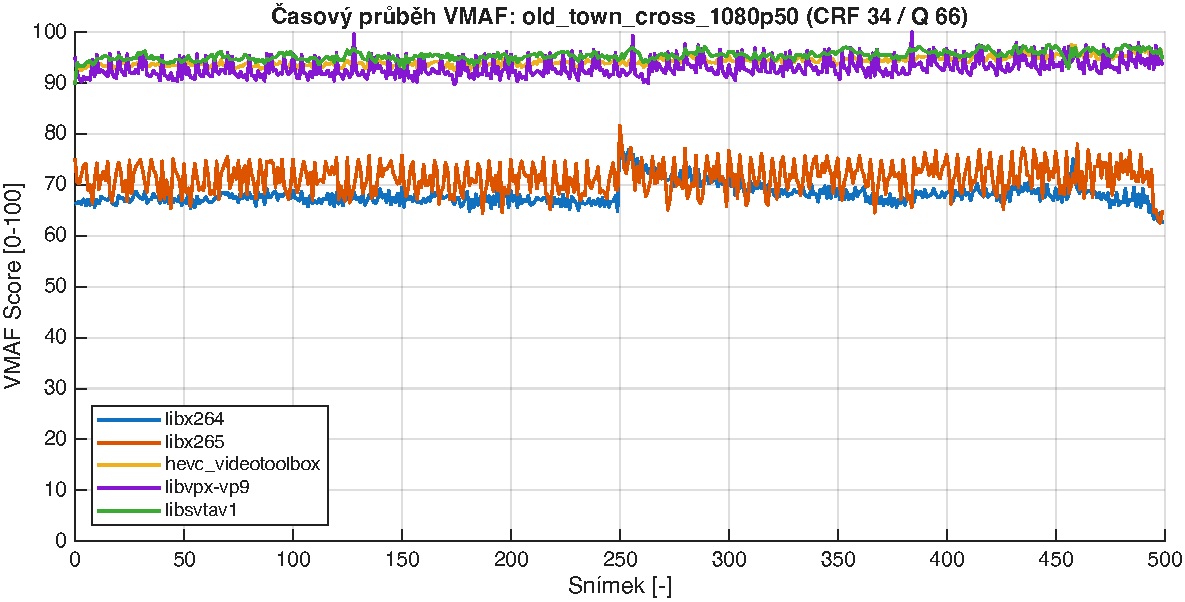
\includegraphics[width=0.85\textwidth]{per_frame_vmaf_old_town_cross_1080p50.pdf}
    \caption{Časový průběh \hyperref[sec:metrics]{VMAF}: old\_town\_cross\_1080p50.}
\end{figure}

\begin{figure}[H]
    \centering
    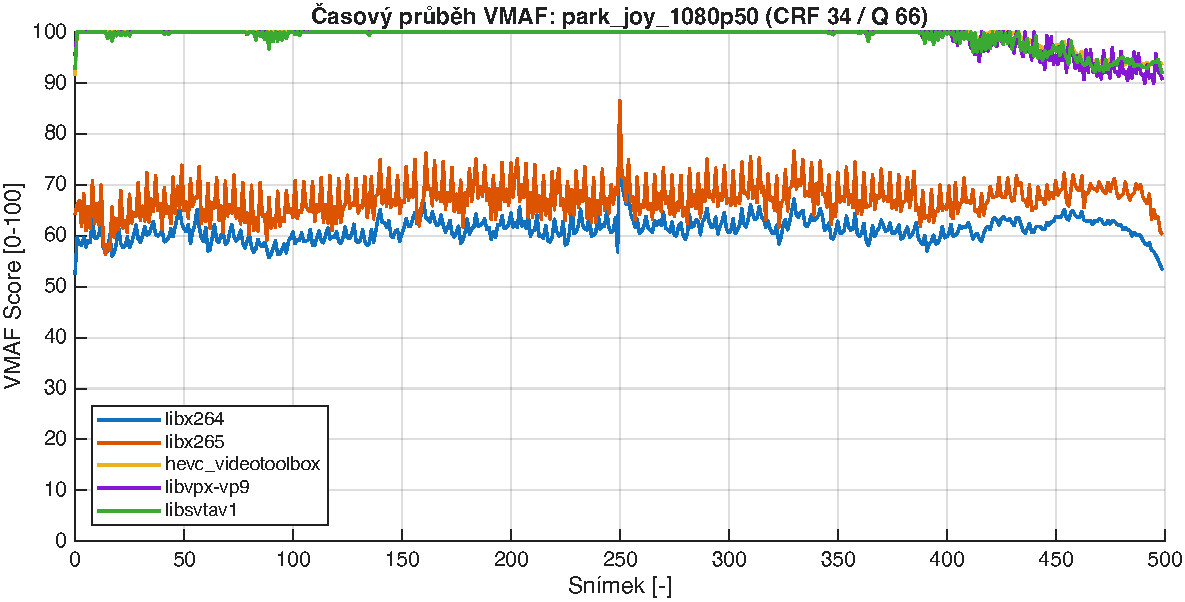
\includegraphics[width=0.85\textwidth]{per_frame_vmaf_park_joy_1080p50.pdf}
    \caption{Časový průběh \hyperref[sec:metrics]{VMAF}: park\_joy\_1080p50.}
\end{figure}

\newpage
\subsection*{R-D Křivky (Rate-Distortion)}
Kompletní sada naměřených RD křivek pro metriky \hyperref[sec:metrics]{PSNR}, \hyperref[sec:metrics]{SSIM} a~\hyperref[sec:metrics]{VMAF} pro zbývající sekvence.

\subsubsection*{Sekvence: crowd\_run\_1080p50}

\begin{figure}[H]
    \centering
    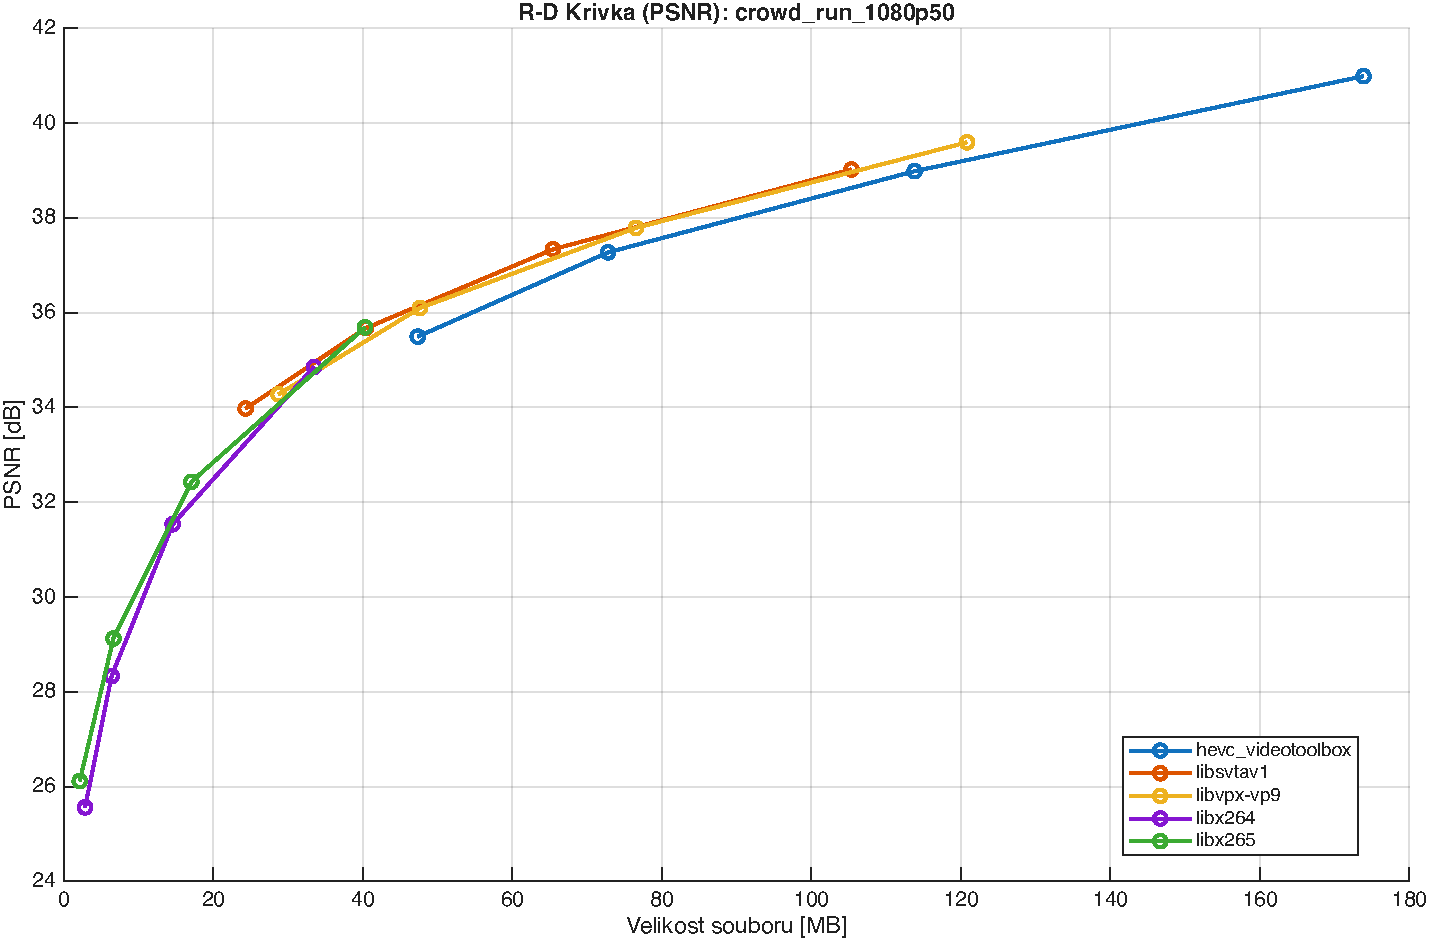
\includegraphics[width=0.75\textwidth]{rd_psnr_crowd_run_1080p50.pdf}
    \caption{R-D Křivka (\hyperref[sec:metrics]{PSNR}) pro sekvenci crowd\_run\_1080p50.}
\end{figure}

\begin{figure}[H]
    \centering
    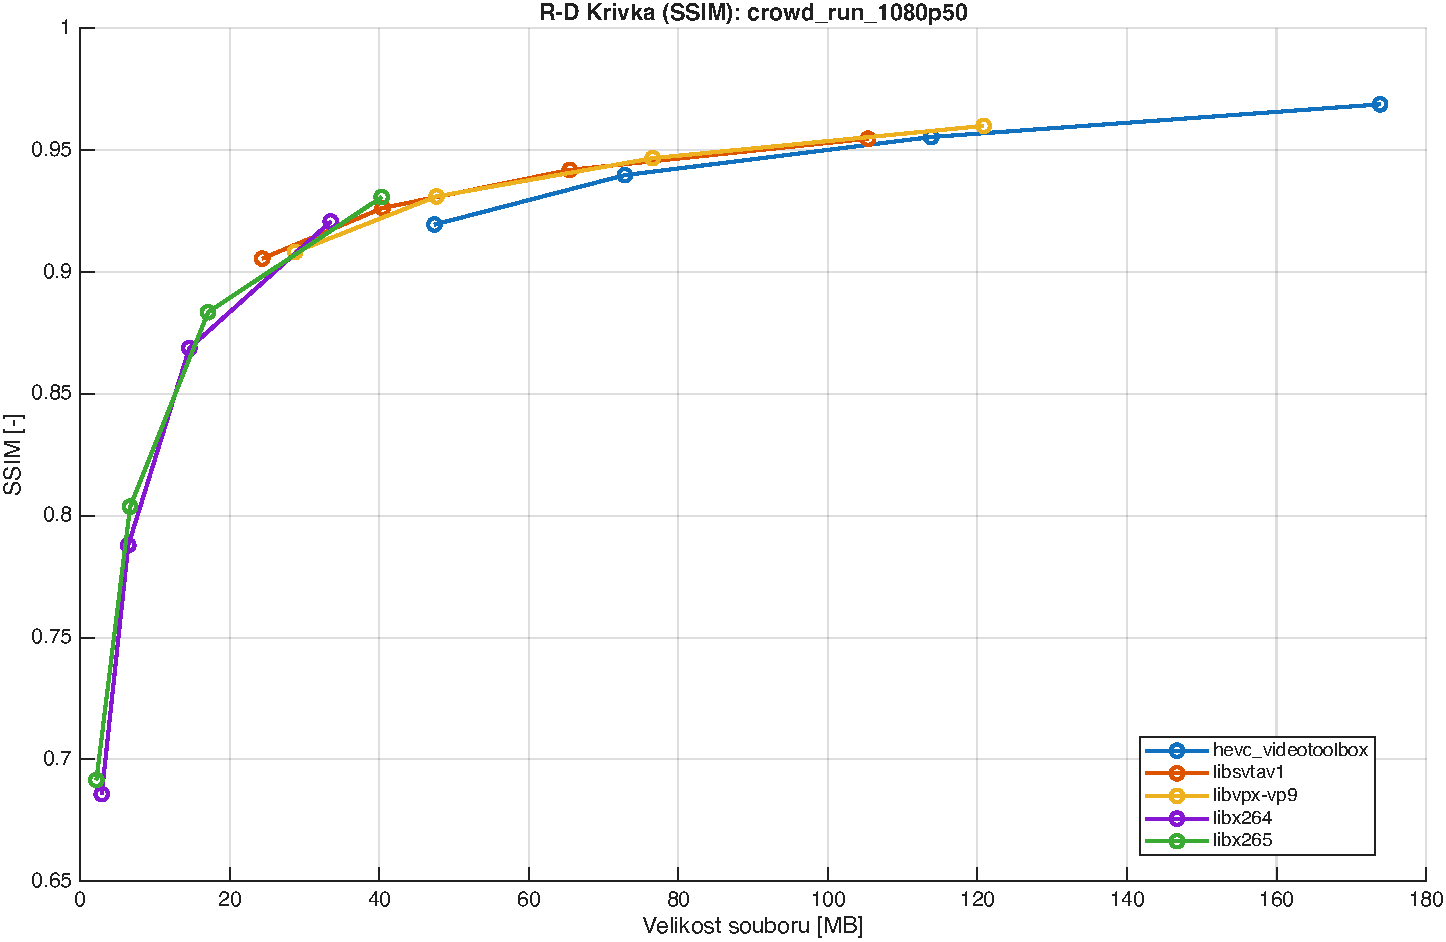
\includegraphics[width=0.75\textwidth]{rd_ssim_crowd_run_1080p50.pdf}
    \caption{R-D Křivka (\hyperref[sec:metrics]{SSIM}) pro sekvenci crowd\_run\_1080p50.}
\end{figure}

\subsubsection*{Sekvence: park\_joy\_1080p50}

\begin{figure}[H]
    \centering
    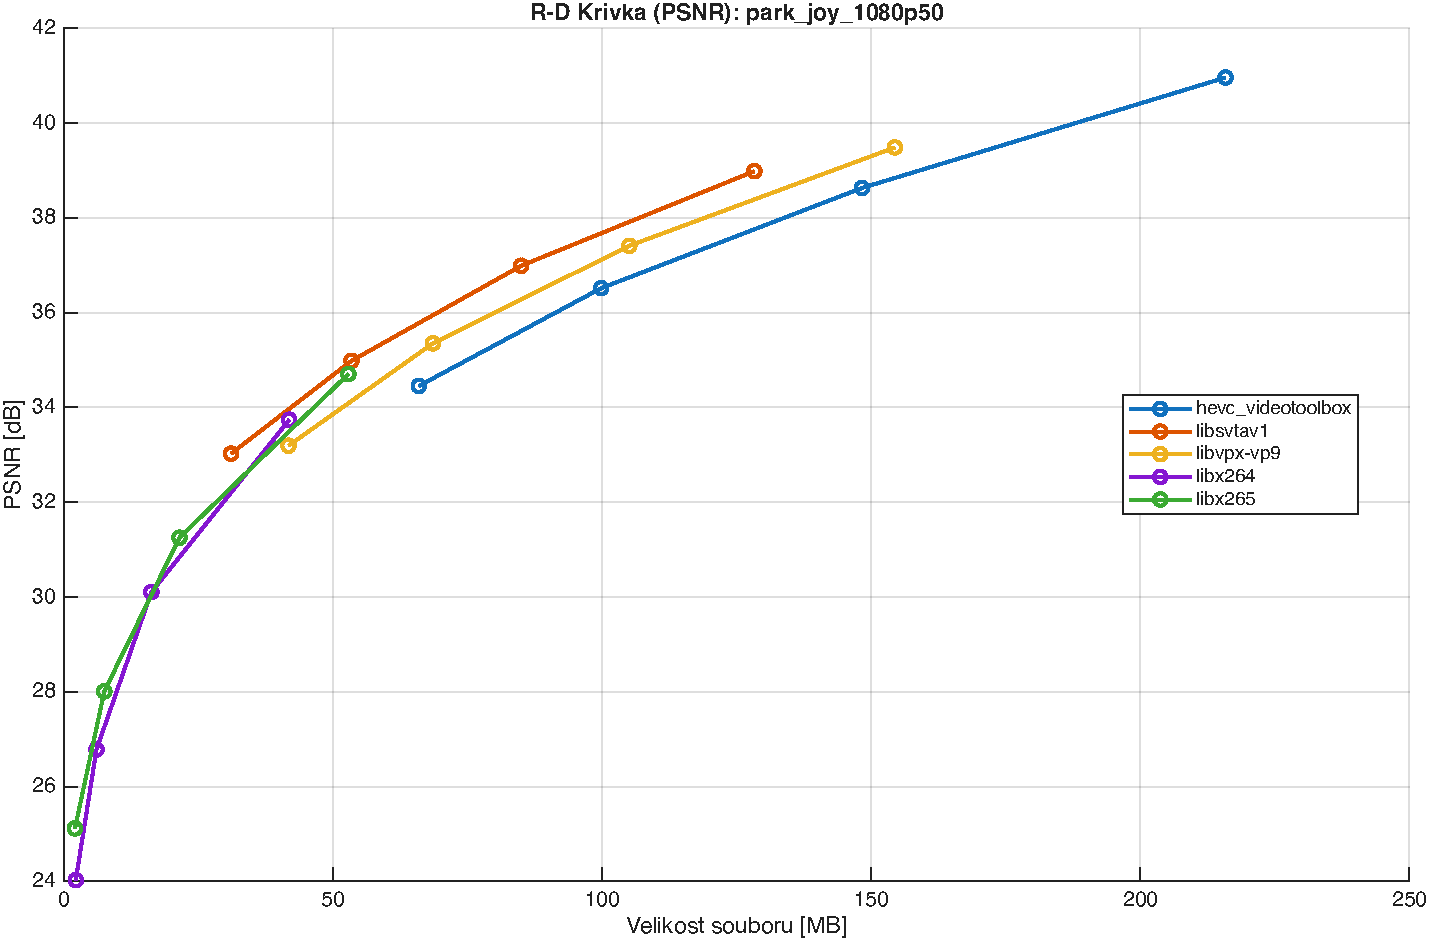
\includegraphics[width=0.75\textwidth]{rd_psnr_park_joy_1080p50.pdf}
    \caption{R-D Křivka (\hyperref[sec:metrics]{PSNR}) pro sekvenci park\_joy\_1080p50.}
\end{figure}

\begin{figure}[H]
    \centering
    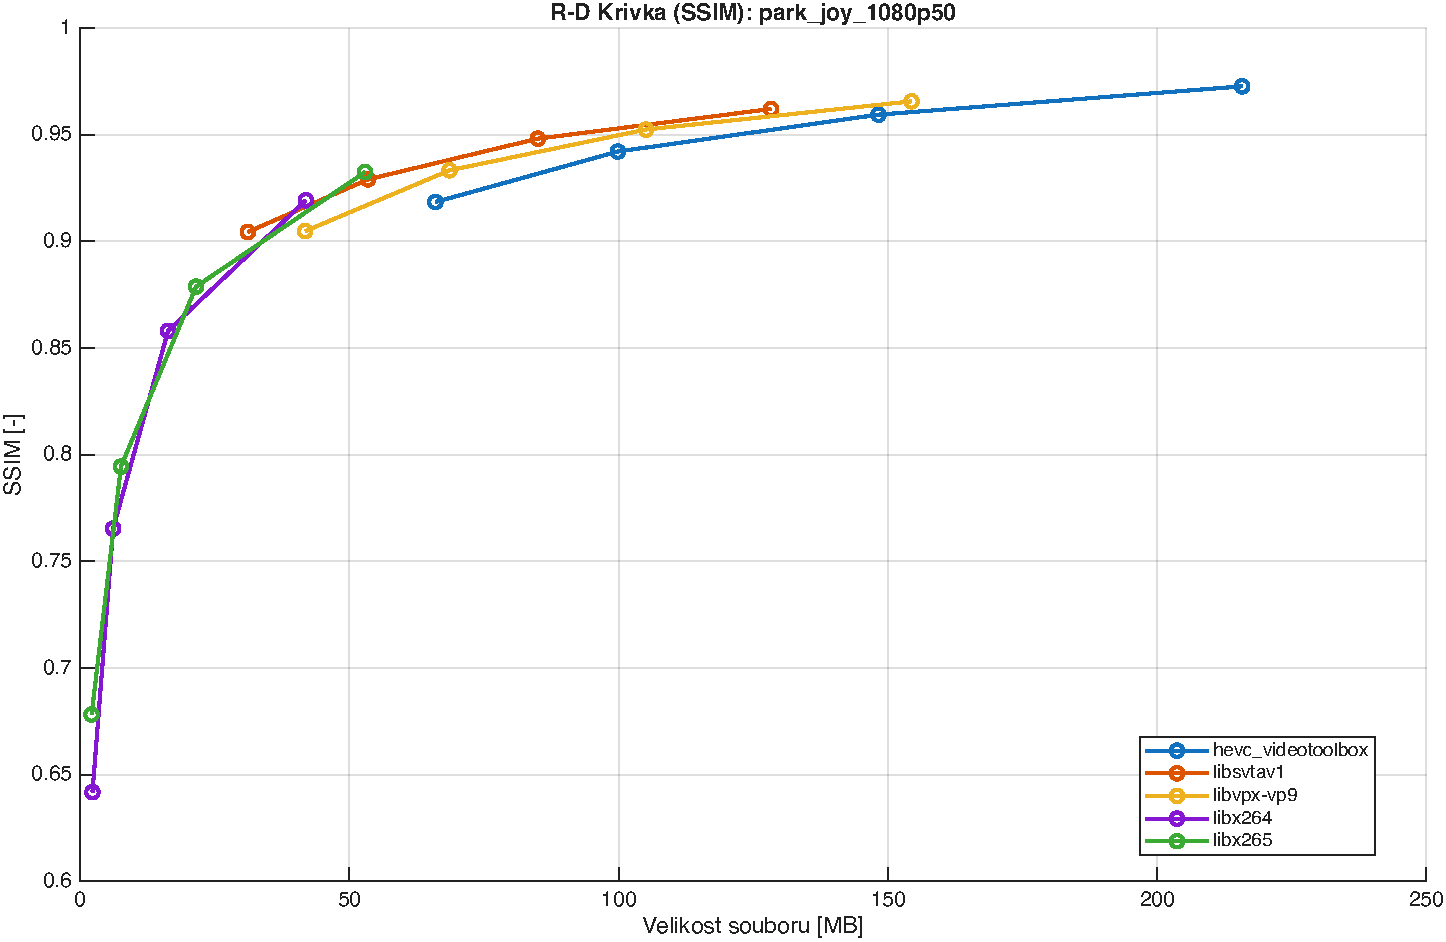
\includegraphics[width=0.75\textwidth]{rd_ssim_park_joy_1080p50.pdf}
    \caption{R-D Křivka (\hyperref[sec:metrics]{SSIM}) pro sekvenci park\_joy\_1080p50.}
\end{figure}

\begin{figure}[H]
    \centering
    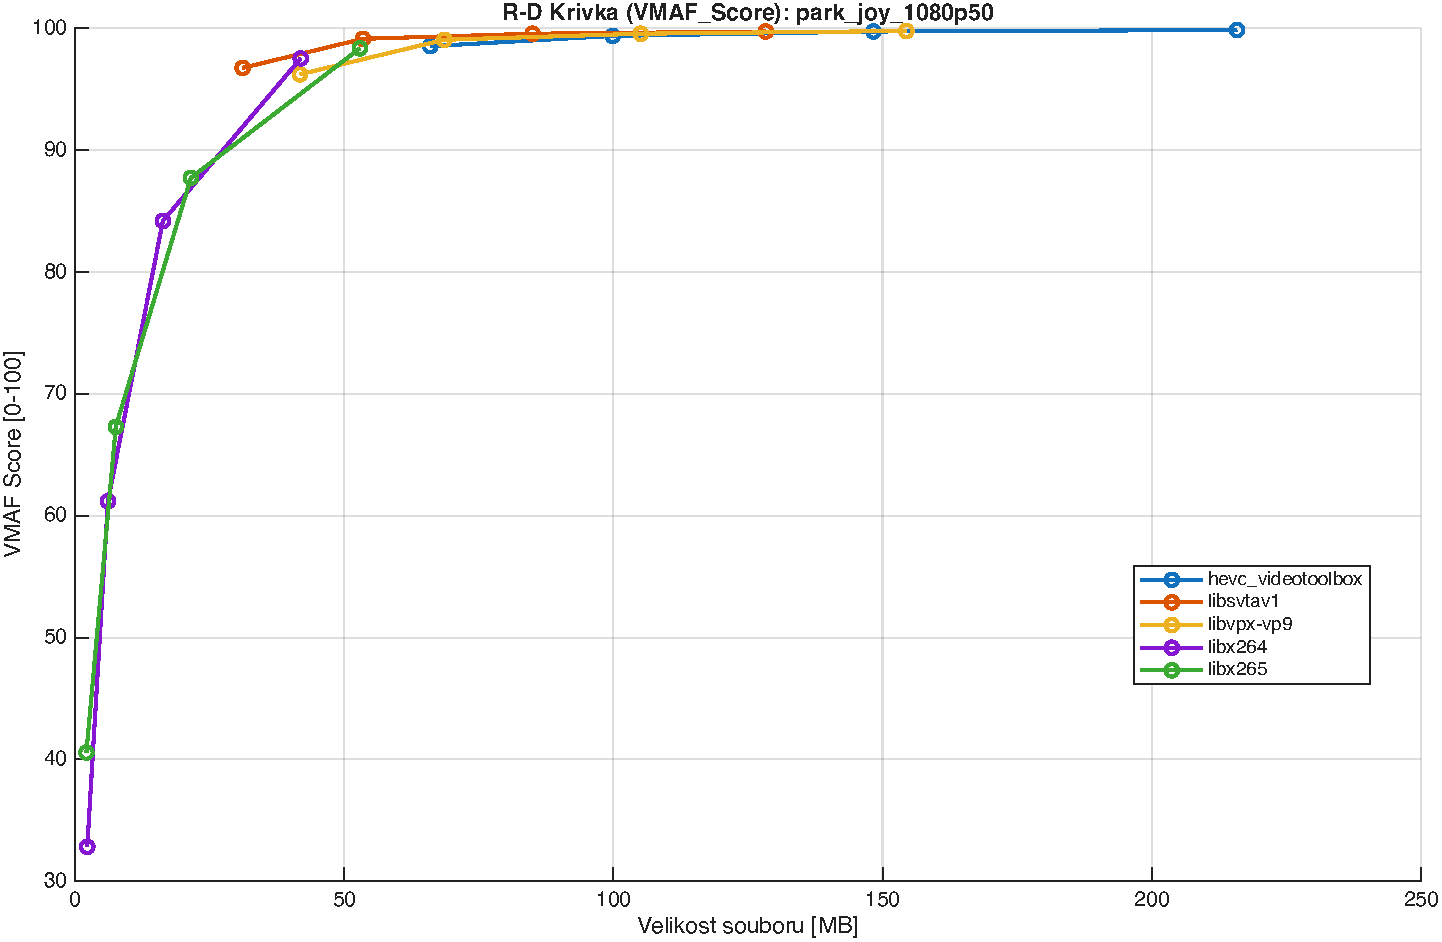
\includegraphics[width=0.75\textwidth]{rd_vmaf_park_joy_1080p50.pdf}
    \caption{R-D Křivka (\hyperref[sec:metrics]{VMAF}) pro sekvenci park\_joy\_1080p50.}
\end{figure}

\subsubsection*{Sekvence: old\_town\_cross\_1080p50}

\begin{figure}[H]
    \centering
    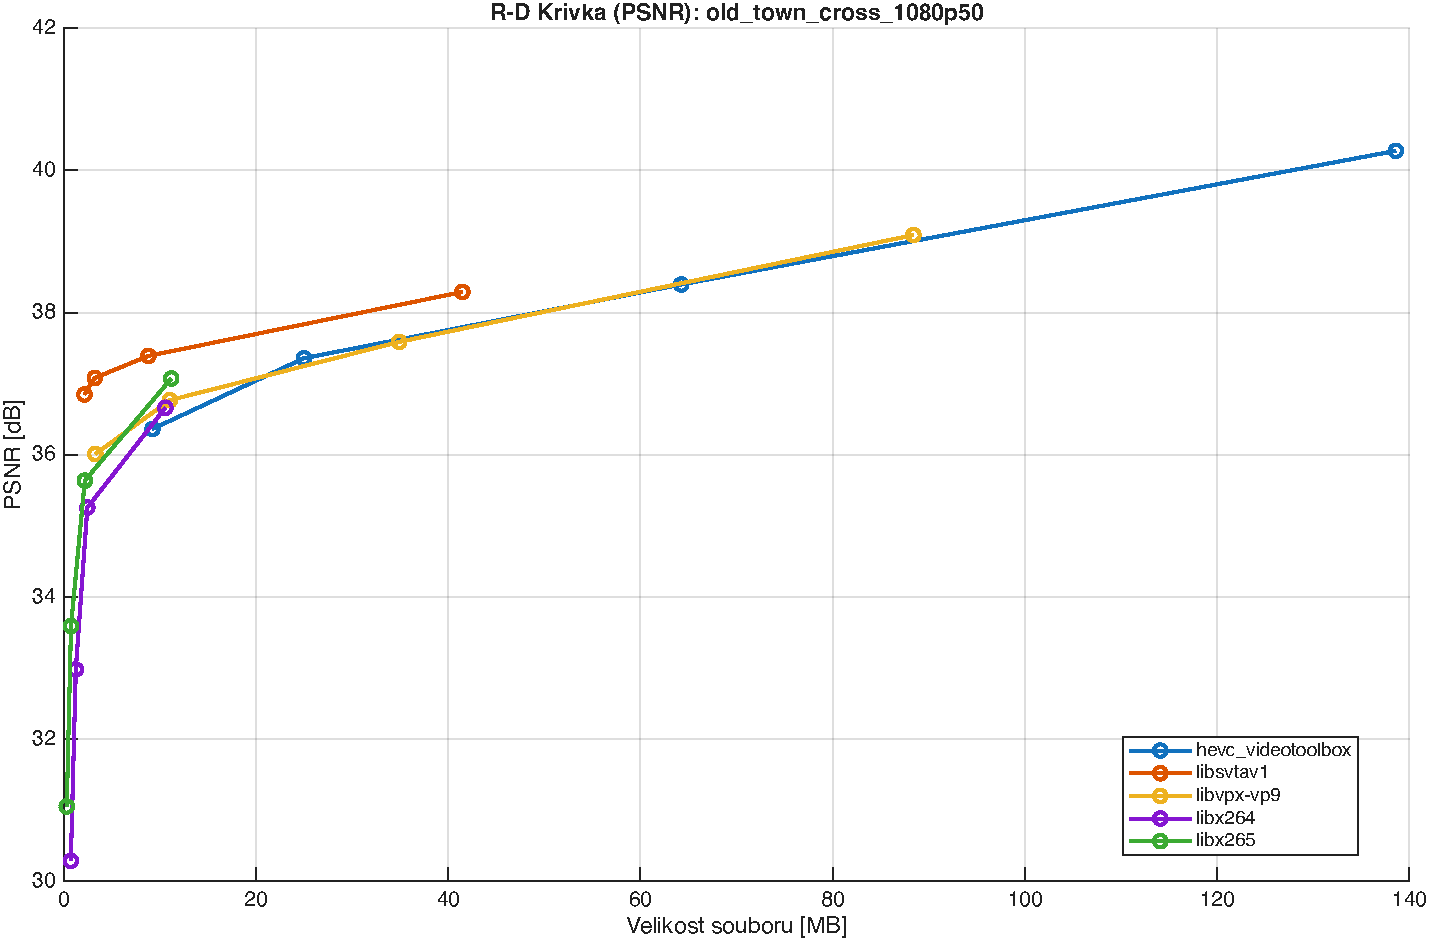
\includegraphics[width=0.75\textwidth]{rd_psnr_old_town_cross_1080p50.pdf}
    \caption{R-D Křivka (\hyperref[sec:metrics]{PSNR}) pro sekvenci old\_town\_cross\_1080p50.}
\end{figure}

\begin{figure}[H]
    \centering
    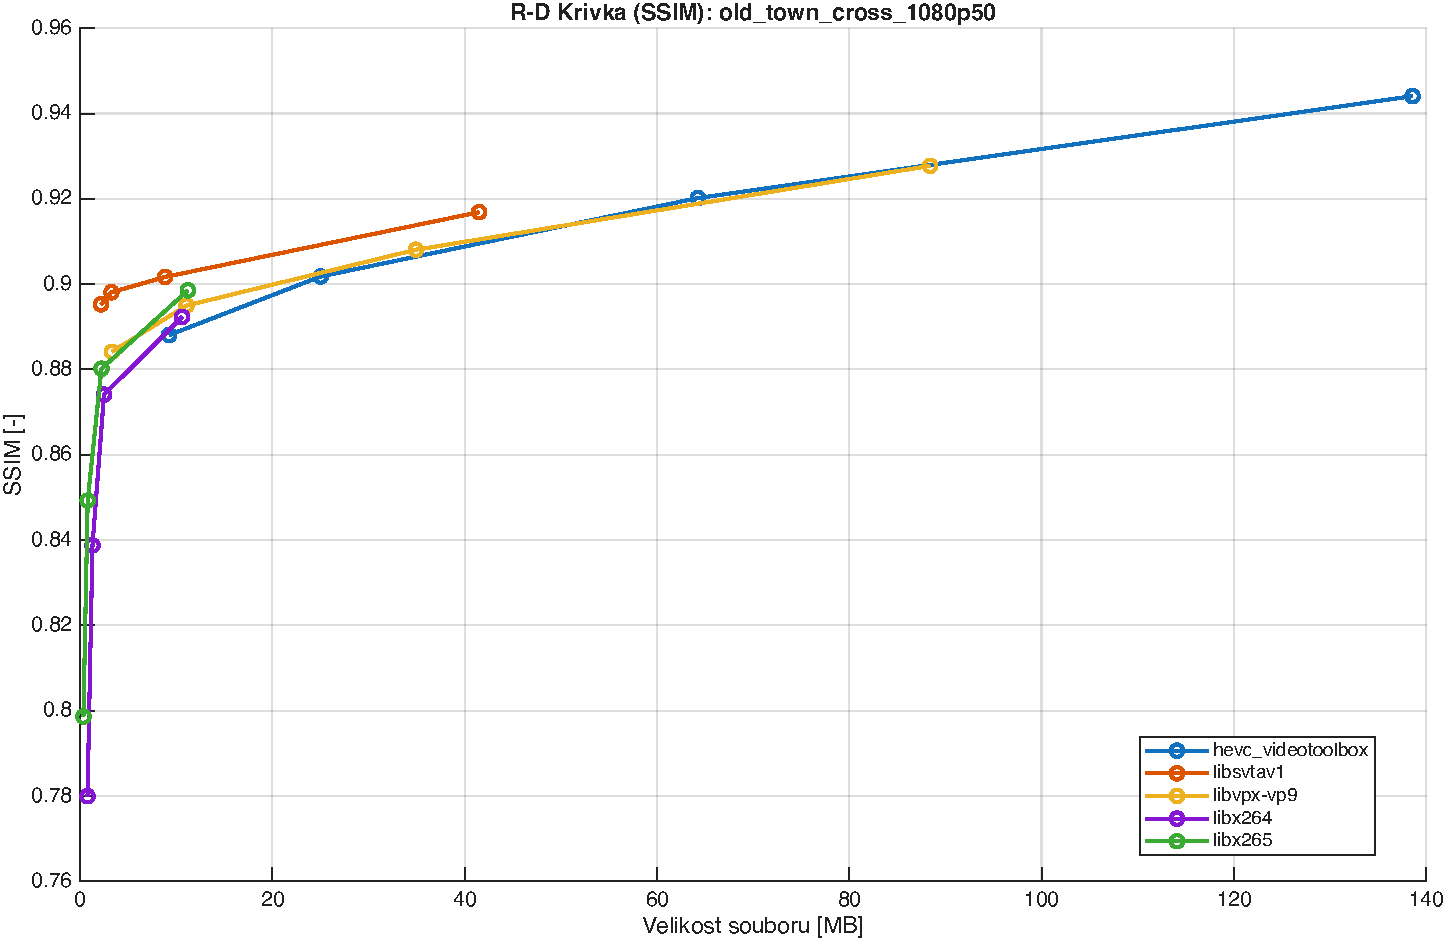
\includegraphics[width=0.75\textwidth]{rd_ssim_old_town_cross_1080p50.pdf}
    \caption{R-D Křivka (\hyperref[sec:metrics]{SSIM}) pro sekvenci old\_town\_cross\_1080p50.}
\end{figure}

\begin{figure}[H]
    \centering
    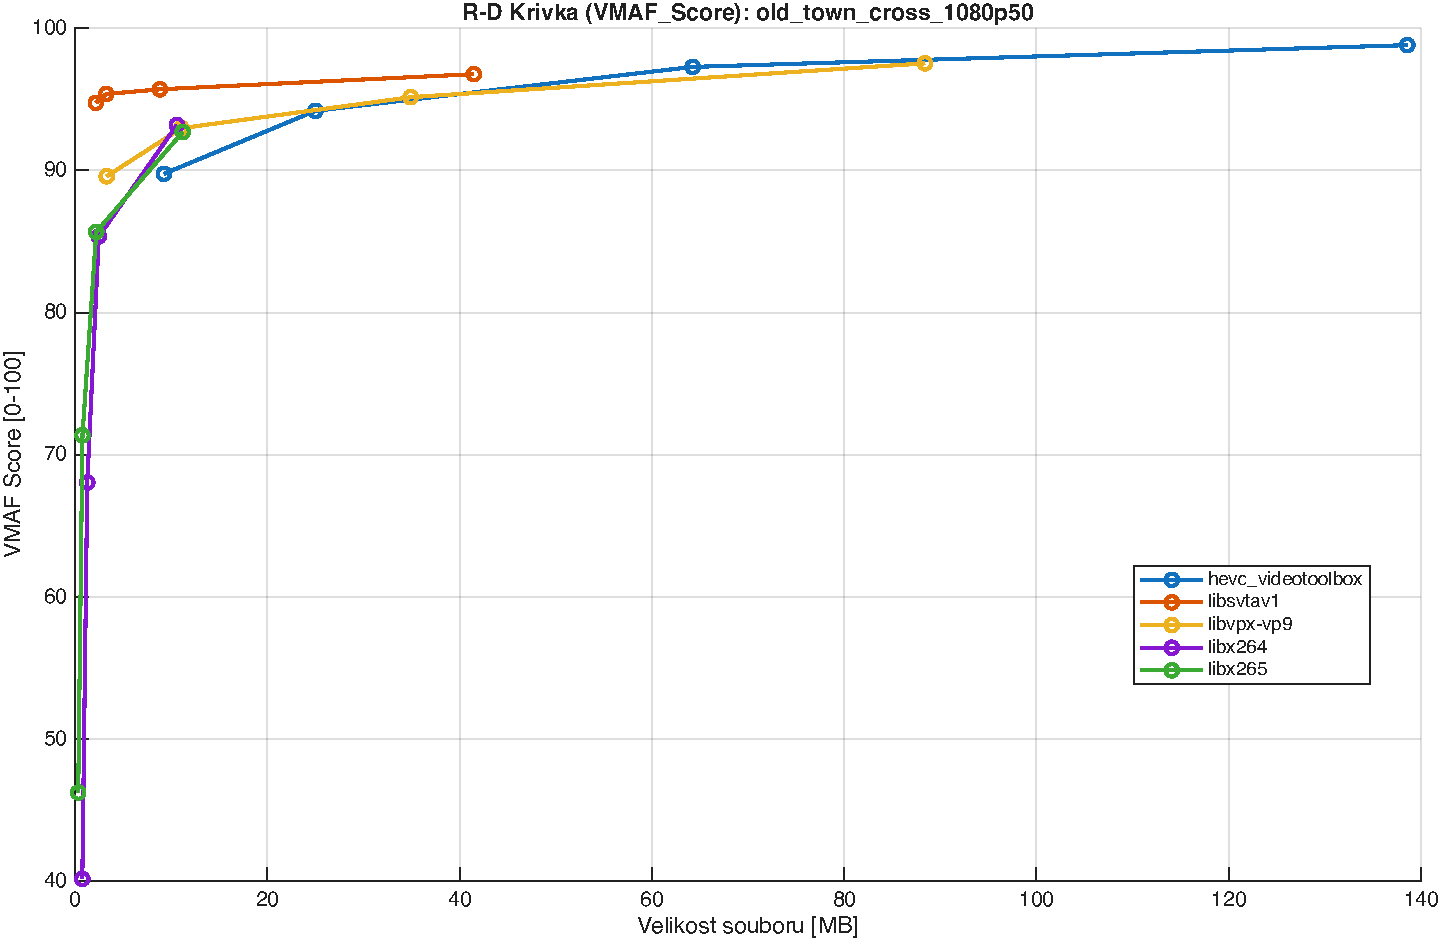
\includegraphics[width=0.75\textwidth]{rd_vmaf_old_town_cross_1080p50.pdf}
    \caption{R-D Křivka (\hyperref[sec:metrics]{VMAF}) pro sekvenci old\_town\_cross\_1080p50.}
\end{figure}

\end{document}